\begin{acquis}
\begin{itemize}
\item nommer un point, une droite, une demi-droite, un segment, un angle;
\item reconnaître des points alignés;
\item tracer la perpendiculaire à une droite passant par un point;
\item tracer la parallèle à une droite passant par un point;
\item tracer la médiatrice d’un segment au compas et coder la figure obtenue;
\item utiliser le rapporteur pour tracer un angle et mesurer un angle;
\item tracer la bissectrice d’un angle au compas et coder la figure obtenue;
\item tracer un cercle connaissant son rayon ou son diamètre;
\item placer des points diamétralement opposés sur un cercle;
\item coder une figure;
\item utiliser la propriété de la médiatrice dans un exercice.
\end{itemize}
\end{acquis} 

\QCMautoevaluation{Pour chaque question, plusieurs réponses sont
  proposées.  Déterminer celles qui sont correctes.}

\begin{QCM}
  \begin{GroupeQCM}
    \begin{exercice}
     Sur la figure ci-contre : \vspace{-2em} \begin{center} 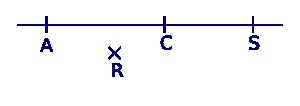
\includegraphics[width=4.3cm]{droiteARCS} \end{center} \vspace{-1em}
      \begin{ChoixQCM}{4}
      \item $R \in [AC]$
      \item $C \in [AC]$
      \item $A \in [CS]$
      \item $S \notin [AC]$
      \end{ChoixQCM}
\begin{corrige}
     \reponseQCM{bd} 
   \end{corrige}
    \end{exercice}
 
    
    \begin{exercice}
     Sur la figure ci-contre : \vspace{-2em}\begin{center}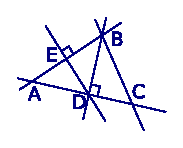
\includegraphics[width=2.5cm]{trianglesABCDE}\end{center}\vspace{-1em}
      \begin{ChoixQCM}{4}
      \item les droites $(ED)$ et $(BC)$ sont parallèles
      \item le point $B$ appartient à la perpendiculaire à $(AC)$ passant par $D$
      \item la droite perpendiculaire à $(AB)$ passant par $D$ coupe $(AB)$ en $E$
      \item le point $A$ appartient à la  perpendiculaire à $(BC)$ passant par $E$
      \end{ChoixQCM}
\begin{corrige}
     \reponseQCM{bc}
   \end{corrige}
    \end{exercice}


    \begin{exercice}
     Dans quel(s) cas, l'équerre est‑elle bien placée pour tracer la perpendiculaire à la droite $d$ passant par le point $A$ ?
      \begin{ChoixQCM}{4}
      \item 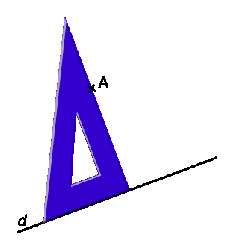
\includegraphics[width=1.8cm]{equerreQCM1}
      \item 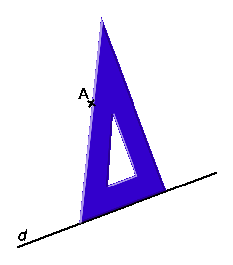
\includegraphics[width=1.8cm]{equerreQCM2}
      \item 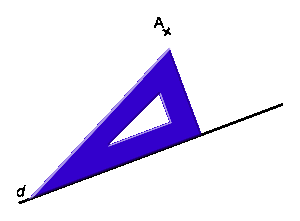
\includegraphics[width=2.4cm]{equerreQCM3}
      \item 
\includegraphics[width=2.4cm]{equerreQCM4}
      \end{ChoixQCM}
\begin{corrige}
     \reponseQCM{a}
   \end{corrige}
    \end{exercice}

   \end{GroupeQCM}  
 \end{QCM}  
 
 
 \begin{QCM}
  \begin{GroupeQCM}  

    \begin{exercice}
     Dans quel(s) cas, les instruments sont‑ils bien placés pour construire la parallèle à la droite $d$ passant par le point $A$ ?
      \begin{ChoixQCM}{4}
      \item 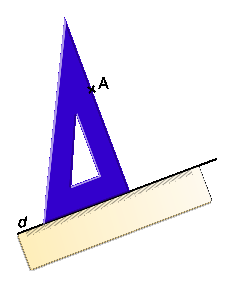
\includegraphics[width=1.8cm]{equerreQCM5}
      \item 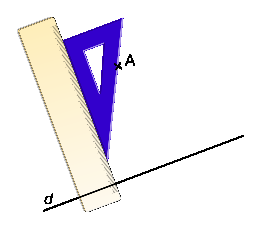
\includegraphics[width=2.4cm]{equerreQCM6}
      \item 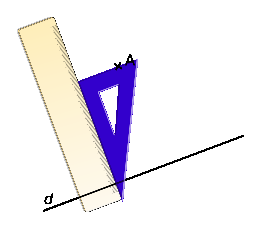
\includegraphics[width=2.4cm]{equerreQCM7}
      \item 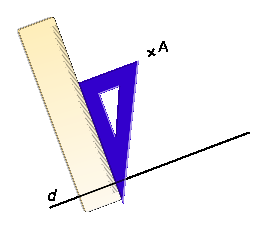
\includegraphics[width=2.4cm]{equerreQCM8}
      \end{ChoixQCM}
\begin{corrige}
     \reponseQCM{c}
   \end{corrige}
    \end{exercice}
  
  
    \begin{exercice}
     Soit $d_1$, $d_2$ et $d_3$ trois droites. Si $d_1 \perp d_2$ et $d_3 \perp d_2$ alors \ldots
      \begin{ChoixQCM}{4}
      \item $d_1$ et $d_3$ sont sécantes
      \item $d_2 \parallel d_3$
      \item $d_1 \perp d_3$
      \item $d_1 \parallel d_3$
      \end{ChoixQCM}
\begin{corrige}
     \reponseQCM{d}
   \end{corrige}
    \end{exercice}
    
    
  \begin{exercice}
     Sur la figure ci-contre : \vspace{-2em}\begin{center}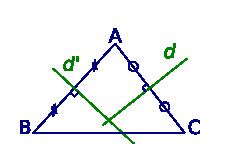
\includegraphics[width=2.9cm]{triangleABCdd}\end{center}\vspace{-1em}
      \begin{ChoixQCM}{4}
      \item $d$ est la médiatrice de $[BC]$
      \item $d$ est la médiatrice de $[AC]$
      \item $d'$ est la médiatrice de $[AB]$
      \item $d'$ est la médiatrice de $[AC]$
      \end{ChoixQCM}
\begin{corrige}
     \reponseQCM{bc}
   \end{corrige}
    \end{exercice}

     \begin{exercice}
     Si $Z$ appartient à la médiatrice de $[ST]$ alors \ldots
      \begin{ChoixQCM}{4}
      \item $ST = ZT$
      \item $ZS = ZT$
      \item $ZS = TS$
      \item $TZ = SZ$
      \end{ChoixQCM}
\begin{corrige}
     \reponseQCM{bd}
   \end{corrige}
    \end{exercice}
    

     \begin{exercice}
     Le point $A$ est le sommet des angles... \vspace{-2em}\begin{center}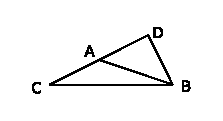
\includegraphics[width=2.6cm]{sommetA}\end{center}\vspace{-1em}
      \begin{ChoixQCM}{4}
      \item $\widehat{ABC}$
      \item $\widehat{BAC}$
      \item $\widehat{DAC}$
      \item $\widehat{BDA}$
      \end{ChoixQCM}
\begin{corrige}
     \reponseQCM{bc}
   \end{corrige}
    \end{exercice}
    
    
     \begin{exercice}
     Un angle mesurant $92^\circ$ est \ldots
      \begin{ChoixQCM}{4}
      \item aigu
      \item obtus
      \item plat
      \item droit
      \end{ChoixQCM}
\begin{corrige}
     \reponseQCM{b}
   \end{corrige}
    \end{exercice}
    
    
     \begin{exercice}
     Sur la figure ci-contre : \vspace{-2em}\begin{center}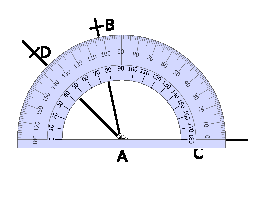
\includegraphics[width=3.8cm]{rapporteurQCM}\end{center}\vspace{-1em}
      \begin{ChoixQCM}{4}
      \item $\widehat{BAC} = 118^\circ$
      \item $\widehat{CAD} = 145^\circ$
      \item $\widehat{CAB} = 102^\circ$
      \item $\widehat{BAD} = 33^\circ$
      \end{ChoixQCM}
\begin{corrige}
     \reponseQCM{cd}
   \end{corrige}
    \end{exercice}
    
    
    \begin{exercice}
     Sur quelle(s) figure(s) la demi-droite orange est-elle la bissectrice de l'angle $\widehat{LIN}$ ?
      \begin{ChoixQCM}{4}
      \item 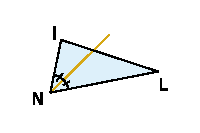
\includegraphics[width=2.2cm]{ddroite-orange1}
      \item 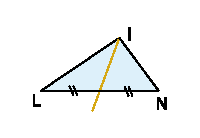
\includegraphics[width=2.2cm]{ddroite-orange2}
      \item 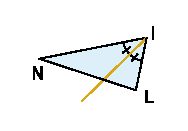
\includegraphics[width=2.2cm]{ddroite-orange3}
      \item 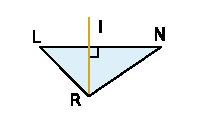
\includegraphics[width=2.2cm]{ddroite-orange4}
      \end{ChoixQCM}
\begin{corrige}
     \reponseQCM{c}
   \end{corrige}
    \end{exercice}
\end{GroupeQCM}
\end{QCM}

  
